\chapter{Logical Normal Form Networks}\label{C:workdone}
Assume the problem we are trying to learn has some boolean formula which underpins it. Then it is known that this formula must have a Conjunctive Normal Form (CNF) or Disjunctive Normal Form (DNF). This section explores networks which learn the CNF or DNF representation of any underlying boolean expression.\\

The paper "Backpropagation for Neural DNF and CNF Networks" \cite{herrmann1996backpropagation} proposes networks which can solve this task, however the paper does not provide justification, consequently it is diffcult to understand and reproduce. This report takes this concept but rederives it using the Noisy-OR and Noisy-AND gates \cite{LearningLogicalActivations}.\\

A CNF or DNF formula contains clauses of literals which is either an atom or a negation of an atom. To account for this the number of inputs to the network will be doubled, i.e. the inputs will be all the atoms and negations of thoughs atoms. $2^n$ is an upper bound on the number of Noisy gates needed to learn any boolean expression of $n$ inputs. To ensure that an LNF Network can learn a boolean expression the number of Noisy gates in the hidden layer will be $2^n$.

\section{Noisy Gate Paramaterisation} 
The paramaterisation of Noisy gates require weight clipping, an expensive operation, to avoid manual clipping a new paramaterisation is derived that implisitley clips the weights. Consider that $\epsilon \in (0, 1]$, therefore let $\epsilon_i = \sigma(w_i)$, these $w_i$'s can be trained without any clipping, after training the origonal $\epsilon_i$'s can be recovered.\\

Now these weights must be substutited into the Noisy activation. Consider the Noisy-OR activation.

\begin{align*}
a(X) &= 1 - \prod^p_{i=1}(\epsilon_i^{x_i}) \cdot \epsilon_b\\
&= 1 - \prod^p_{i=1}(\sigma(w_i)^{x_i}) \cdot \sigma(b)\\
&= 1 - \prod^p_{i=1}((\frac{1}{1 + e^{-w_i}})^{x_i}) \cdot \frac{1}{1 + e^{-b}}\\
&= 1 - \prod^p_{i=1}((1 + e^{-w_i})^{-x_i}) \cdot (1 + e^{-w_i})^{-1}\\
&= 1 - e^{\sum^p_{i=1} ln(1 + e^{-w_i}) + ln(1 + e^{-b})} \\
&Let\ w_i^{'} = ln(1 + e^{-w_i}),\ b^{'} = ln(1 + e^{-b})\\
&= 1 - e^{-(W^{'} \cdot X + b^{'})}
\end{align*}

From a similar derivation we get the activation for a Noisy-AND, concisely giving equations \ref{equ:real-noisy-and-activation}, \ref{equ:real-noisy-or-activation}

\begin{align}
a_{and}(X) &= e^{W^{'} \cdot (1 - X) + b^{'}} \label{equ:real-noisy-and-activation}\\
a_{or}(X)&= 1 - e^{-(W^{'} \cdot X + b^{'})} \label{equ:real-noisy-or-activation}
\end{align}

The function taking $w_i$ to $w_i^{'}$ is the soft ReLU function which is peforming a soft clipping on the $w_i$'s. 

\section{Training LNF Networks}
Using equations \ref{equ:real-noisy-or-activation} and \ref{equ:real-noisy-and-activation} for the Noisy-OR, Noisy-AND activations retrespectively allows the networks to be trained without expliscit clipping. The ADAM Optimizer is used for training firstly for the convenience of an adaptive learning rate but also because it inclueds the advantages of RMSProp which works well with on-line (single-example-training) learning, which these LNF Networks respond well to.\\

Preliminary testing showed that LNF Networks are able to learn good classifiers on boolean gates, i.e. NOT, AND, NOR, NAND, XOR and Implies. It is also possible to inspect the trained weights and see that the networks have learnt the correct CNF or DNF representation.

\section{LNF Network Peformance}
How do LNF Networks peform against standard perceptron networks which we know to be universal function approximators. Two different perceptron networks will be used as a benchmark, one with the same configuration as the LNF Network, the other with less hidden neurons. The testing will consist of selecting 5 random boolean expressions for $2 \leq n \leq 9$ and training each network 5 times, each with random initial conditions. Figure \ref{fig:peformance-comparason-all} shows a comparason between all 4 of the networks and figure \ref{fig:peformance-comparason-cnfdnf} shows just the LNF Networks.

\begin{figure}[H]
  \centering
  \begin{minipage}[b]{0.8\textwidth}
    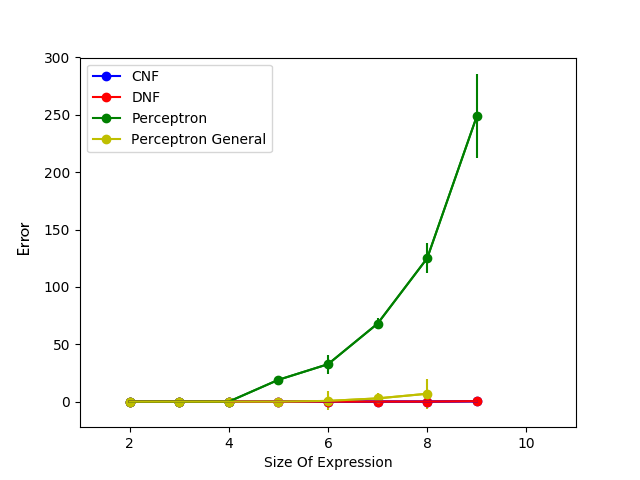
\includegraphics[width=\textwidth]{All-Peformance-Comparason.png}
    \caption{}
    \label{fig:peformance-comparason-all}
  \end{minipage}
  \hfill
\end{figure}

\begin{figure}[H]
  \centering
  \begin{minipage}[b]{0.8\textwidth}
    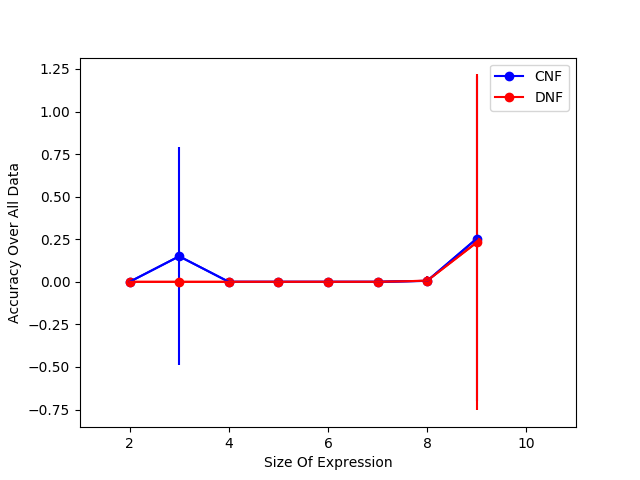
\includegraphics[width=\textwidth]{CNFvsDNF.png}
    \caption{}
    \label{fig:peformance-comparason-cnfdnf}
  \end{minipage}
  \hfill
\end{figure}

Figure  \ref{fig:peformance-comparason-all} shows that neither of the perceptron networks peform as well as the LNF Networks as $n$ increases. Figure  \ref{fig:peformance-comparason-cnfdnf} shows on avarage there are no stastically significant differences between the CNF or DNF networks. What is not present in  \ref{fig:peformance-comparason-cnfdnf} is that at $n = 9$ sometimes the CNF network far out peforms the DNF and visa versa, theoretically both should beable to learn any boolean expression. 

\section{LNF Network Rule Extraction}
The goal of this report is to make neural networks more intepretable, for LNF Networks to addres this problem there must be a way to extract rules from them. Take the weights of a trained LNF Network, these weights can be converted back into $\epsilon_i$'s by apply the sigmoid function to each $w_i$.\\

As $\epsilon_i \rightarrow 0$ then $x_i$ becomes relevent and as $\epsilon_i \rightarrow 1$ then $x_i$ becomes irrielevent. If the network has learnt the correct DNF or CNF representation the for every neuron if input $i$ is relevent then $w_i \rightarrow -\infty$ and therefore $\epsilon_i \rightarrow 0$, othwerwise $x_i$ is irelevent and  $w_i \rightarrow \infty$ meaning $\epsilon_i \rightarrow 1$.\\

Consequently in $\epsilon$ form the network is binary and rules can be easily extracted. Many of the formulas extracted contain redundent terms, i.e. clauses that are a tautologie or a duplicate of another, filtering these out is not an expensive operation.\\

When training an LNF network over the entire truth table for a boolean expression, when a low error is achieved it is possible to extract boolean formula from the network which gets can generate the origonal truth table. This is a necessary first step but a more important question is, can formula still be extracted from the network when the LNF network is not trained with the entire truth table?

\section{LNF Network Generalization}
These networks are able to peform as well as standard perceptron networks but so far they have been getting the complete set of data, in practice this will almost never be the case. Perceptron networks are so widely used because of their ability to generalize, for LNF Networks to be useful they must also be able to generilize.

\begin{figure}[H]
  \centering
  \begin{minipage}[b]{0.8\textwidth}
    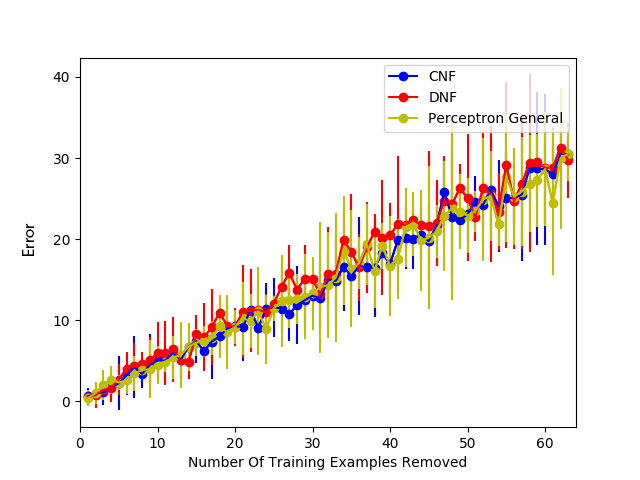
\includegraphics[width=\textwidth]{6-generalization.png}
    \caption{}
  \end{minipage}
 \label{fig:generalization-peformance-6}
  \hfill
\end{figure}

Figure \ref{fig:generalization-peformance-6} shows a comparason between the generalization ability of CNF, DNF and Perceptron networks. The graph shows the peformance over all training data when successively removing elements from the training set. It demonstraits that the CNF and DNF networks generalize as well as the perceptron networks when the boolean formula has 6 inputs.

\subsection{Rule Extraction}
